\documentclass[xcolor=table]{beamer}
\usepackage{comment}
\usetheme{Madrid}
\usepackage{wrapfig}


\title{Recognition and Interactions of Drugs}

% A subtitle is optional and this may be deleted
\subtitle{Advanced Human Languages Technologies}

\author{Pau~Rodriguez \and Asaf~Badouh}

\institute[]
{
  Universitat Politecnica de Catalunya\\
  MIRI - Data Science
  }

\date{May 2018}

\subject{}

\pgfdeclareimage[height=0.5cm]{Logo_UPC}{Logo_UPC}
\logo{\pgfuseimage{Logo_UPC}}

\begin{comment}
\AtBeginSection[]
{
  \begin{frame}<beamer>{Outline}
    \tableofcontents[currentsection]
  \end{frame}
}
\end{comment}
\begin{comment}

ko - introduction
ko - Approach taken to each of the tasks
Used learner(s) (CRF, SVM, ANN, ...), features, architecture, etc.
Used software
Performed experiments
\end{comment}

\begin{document}

\begin{frame}
  \titlepage
\end{frame}

\begin{frame}{Outline}
  \tableofcontents
\end{frame}

% toc; we are going to present our work on Drug Name recognition and Drug Drug Interaction by a general approach overview, the architecture, some detail of the features and the experiments performed

\section{Introduction}
\begin{frame}{Introduction}

Drug name recognition (DNR) is a critical step for drug information extraction.
DNR is the first step to identifying unknown drug interactions (DDI).
DDI is broadly described as a change in the effects of one drug by the presence of another drug.
Because of the lack of labeled corpora, early studies on DNR are mainly based on ontologies and dictionaries.
To promote the research on drug information extraction, MAVIR research network and University Carlos III of Madrid in Spain organized two challenges successively: \textbf{DDIExtraction 2011} and \textbf{DDIExtraction 2013}. 
Both of the two challenges provide labeled corpora that can be used for machine learning-based DNR.\\
We are presenting several approaches to solve \textbf{SemEval-2013 Task 9.1 and Task 9.2}. 
\end{frame}

% We are solving the tasks 9.1 and 9.2 of the SemEval-2013 competition


% \section{Approach} 
% \begin{frame}{Approach taken}
%     \begin{itemize}
%     \item {
%     \textbf{Drug Name Recognition:}
%     }
%       \begin{itemize}
%       \item {
%         Transform and parse the input XML data into new user friendly data base (Json based).
%       }
%       \item {
%         For each word - create Features vector with information we extract based on the data.
%       }
%       \item {
%         Train and examine different learners (SVM and CRF).
%       }
%       \end{itemize}
    
    

%     \item {
%     \textbf{Drug-Drug Interaction:}
%     }
%       \begin{itemize}
%       \item {
%         Parse the input XML data into new user friendly data base (Json based).
%       }
%       \item {
%         Filter out sentences with more than one Drug entity and create features vector.
%       }
%       \item {
%         Train and examine using SVM.
%       }
%       \end{itemize}

    
    
%     \item {
%     \textbf{Sources of inspiration:}
%     }
%       \begin{itemize}
%       \item {
%         Reference papers.$^{\cite{liu_tang_chen_wang_fan_2015,kim_liu_yeganova_wilbur_2015,ratinov_roth_2009,liu_tang_chen_wang_2015}}$
%       }
      
%       \end{itemize}
%     \end{itemize}

% \end{frame}


\section{Approach} 
\begin{frame}{Approach taken}

    \textbf{Overview:}
    \begin{block}{}
    {
        Transform and parse the input XML data into new user friendly data base (Json based).
    }
    \end{block}
    \begin{block}{}
    \begin{itemize}
      \item {\textbf{Drug Name Recognition:}
        For each word - create Features vector with information we extract.
      }
      \item {\textbf{Drug-Drug Interaction:}
        For each Drug pair in sentence - Create feature vectors.
      }
    \end{itemize}
    \end{block}
    \begin{block}{}
        Train and examine different learners (SVM and CRF).
     \end{block}
    \begin{itemize}
    \item {
    \textbf{Sources of inspiration:}
    }
      \begin{itemize}
      \item {
        Reference papers.$^{\cite{liu_tang_chen_wang_fan_2015,kim_liu_yeganova_wilbur_2015,ratinov_roth_2009,liu_tang_chen_wang_2015}}$
      }
      \end{itemize}
    \end{itemize}

\end{frame}
 
% We are training several models, but for each one we use the same general approach: parsing the data, generating a set of features then training the model. The different sets of features for each task are inspired on papers that present solutions to these tasks.

\section{Architecture}
\begin{frame}{Solution's Architecture}
\begin{figure}
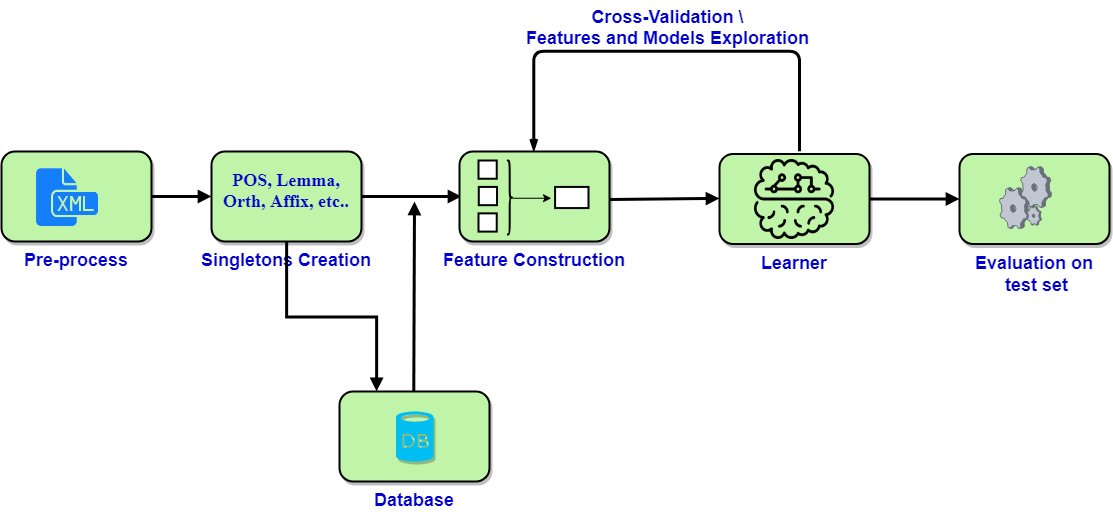
\includegraphics[scale=0.3]{ProcessCV.png}
\end{figure}
\vspace*{-15pt}
\scalebox{0.8}{
\begin{tabular}[c]{@{}ll}
Learners: & Software: \\
 Support Vector Machine (linear kernel) & \small{Scikit-Learn, sklearn-crfsuite}\\
 Conditional Random Fields & \small{Freeling, NLTK, DrugBank$^{\cite{DrugBank}}$, PubMed$^{\cite{PubMedWord2Vec,PubMedDatabase}}$} \\
                           & \small{PyStatParser, Maltparser}\\
\end{tabular}
}
\end{frame}

% Our implementation for each task is based on the same architecture. 
% A component to preprocess data, parsing xml files, 
% A component to generate single word features (token, pos, lemma, orthographic) . More complicated features (or requiring more space) are also saved to disk for further preprocessing or for final model training.
% A component constructs the feature vectors from the features in previous components and in disk, by directives on configuration files.
% Machine learning models are also configured and trained acording to the configuration directives
% Due to our limitations on time and computation power, we performed feature selection and model selection over trainign and test set. This should be redone by doing features selection independently of the model and using crossvalidation over the training set for model selection, before predicting on the testing set.
% we save their results (batch files) on the model configuration files in order to automatically create a report of model scores.

% The software we used is..
% the learners we used are..


%----------------------------------------------------------------------------------------
\section{Features}
\begin{frame}{Features}

\begin{table}[]
\centering
\scalebox{0.8}{
\begin{tabular}{lcl}
\multicolumn{3}{l}{DNR features}                                                                                                               \\ \hline
$f_{1}$ & Word feature             &                                                                                                                               \\
\rowcolor[HTML]{DAE8FC} 
$f_{2}$ & Part-Of-Speech           &                                                                                                                               \\
$f_{3}$ & Lemmatization           &                                                                                                                               \\
\rowcolor[HTML]{DAE8FC} 
$f_{4}$ & Orthographic - basic features     & \begin{tabular}[c]{@{}l@{}}5 classes: \\ all-capitalized, is-titlecase,all-digits,\\ alphanumeric, hyphen or not\end{tabular} \\
$f_{5}$ & Orthographic - affix features           & Prefixes and suffixes of the length 3,4,5                                                                                     \\
\rowcolor[HTML]{DAE8FC} 
$f_{6}$ & Orthographic - Word shape features      & \begin{tabular}[c]{@{}l@{}}Generalized word class: Xxxxx00xxOxx \\ Brief word class: Xx0xOx\end{tabular}                      \\

$f_{7}$ & Dictionary features      & Lookup on Drugbank                                                                                            \\
\rowcolor[HTML]{DAE8FC} 
$f_{8}$ & Chunk feature            &    NLTK noun phrase chunking tag                                                                                                                         \\
$f_{9}$ & Word Embeddings features & Word2Vec and classification                                                                                                  
\end{tabular}}
\end{table}
\end{frame}

% we present now, the single word features we have implemented and tested. Word, lemma, POS tag, common orthographic features. We also implemented Drug dictionary lookup, noun phrase chunking and word2vec.





\begin{frame}{Features}

\begin{table}[]
\centering
\scalebox{0.8}{
\begin{tabular}{lll}
\multicolumn{3}{l}{Drug-Drug Interaction Features}                                       \\ \hline

$f_{1}$ & All DNR SVM features        & for each entity of the pair   \\
\rowcolor[HTML]{DAE8FC} 
$f_{2}$ & All DNR SVM features in a window        & \begin{tabular}[c]{@{}l@{}}for each word  \\ in a window 0 to 5 \end{tabular}                      \\
$f_{3}$ & Appearance of most frequent 3-gram sequences & from dependency tree shortest path    \\
\rowcolor[HTML]{DAE8FC} 
$f_{4}$ &  Appearance of most frequent Word/Lemma  &        \\
$f_{5}$  & Appearance of most frequent POS  & from CFG parse tree shortest path    \\
\rowcolor[HTML]{DAE8FC} 
$f_{6}$ &  Word count in the shortest path  & from dependency tree shortest path        \\
$f_{7}$ &  Counts of POS tags in sentence   &  specific tags: VB, CC, MD, DT

\end{tabular}}
\end{table}
\end{frame}


% We also generated more contextual features for the drug drug interaction task, where we reused the previously seen features and combined them with features related to the sentence and to the sentence's parse trees (dependency and cfg parse tree).


\begin{frame}{Features}{Task9.1 DNR - SVM}

Word embedding features based on Word2Vec model, We used pre-processed database from Pubmed$^{\cite{PubMedDatabase}}$.

\begin{itemize}
    \item Vector feature:
    \begin{itemize}
        \item  Word mapped to 200 dimension vector: (0.010, ..., 0.023)
        \item Failed to train the model due to hardware limitations.
    \end{itemize}
    \item Word cluster feature:
    \begin{itemize}
        \item Use Kmean to cluster words based on their vectors.
        \item Reduce the feature from 200 dimension to 1.
        \item Failed to do the clustering due to hardware limitation.
    \end{itemize}
\end{itemize}
\end{frame}

% Let's show the detail of what we tried for word embeddings. We used this feature in the Drug Name Recognition task.
%Pyysalo et al. (2013)


\begin{frame}{Features}{Task9.2 DDI - Dependency Tree}
\begin{figure}
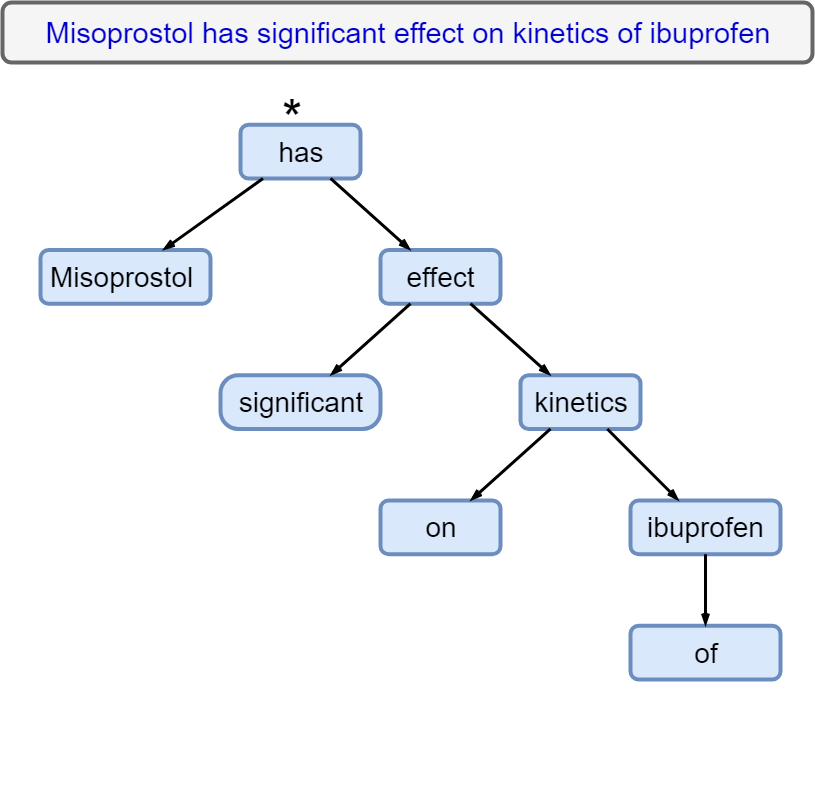
\includegraphics[scale=0.2]{tree.png}
\end{figure}
\vspace*{-35pt}
\small{ShortestPath(Misoprostol, ibuprofen) = [has, effect, kinetics]\\
LenthOfShortestPath = 3\\
3-grams: [Misoprostol, has, effect],[has, effect, kinetics], [effect, kinetics, ibuprofen]}
\end{frame}

% for the contextual features, Used in the drug drug interaction task, we created different parse trees (Dependency and CFG). Here we have an example of a dependency tree in a sentence with 2 drugs. We extract the shortest path from the parse tree for each pair interaction and sentence. Then for each shortest path we extract the trigrams, words, lemma , pos and we count how many times each of them appears in the whole training data set. Finally we keep the more frequent one with a specific threshold (50 for memory reasons). And finally the feature for each pair- sentence will be the binary var that indicates each fo the frequent words/trigrams/etc is in the sentence's shortest path or not.


\begin{frame}{Features}{Task9.1 DNR - SVM}
Based on the singleton features, we explore different combinations of vectors to feed the learners:
\begin{figure}
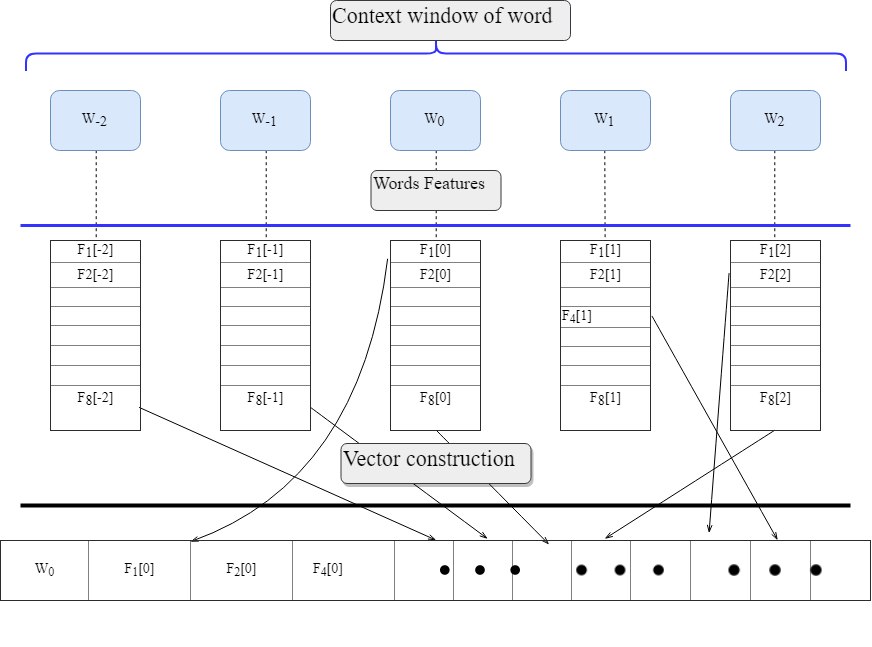
\includegraphics[scale=0.3]{VectorConstruction.png}
\end{figure}
\end{frame}

% in this schema we can see a word within the dataset with its features and the features of the word around it in a window of 2. All the features are used to construct a feature vector for each word of the data set.
% this is the feature structure used in task 9.1 with the linear SVM learning algorithm




\begin{frame}{Features}{Task9.1 DNR - CRF}
\begin{figure}
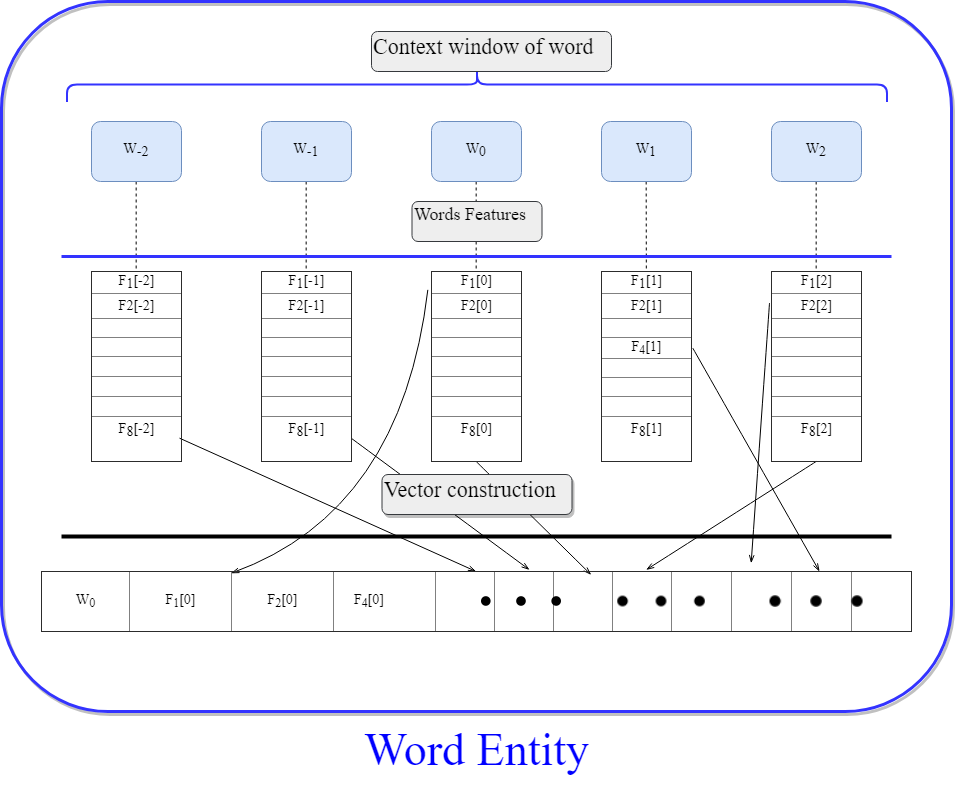
\includegraphics[scale=0.25]{wordEntity.png}
\end{figure}
\end{frame}


% the previous single word features can be considered a single component.

\begin{frame}{Features}{Task9.1 DNR - CRF}
\begin{figure}
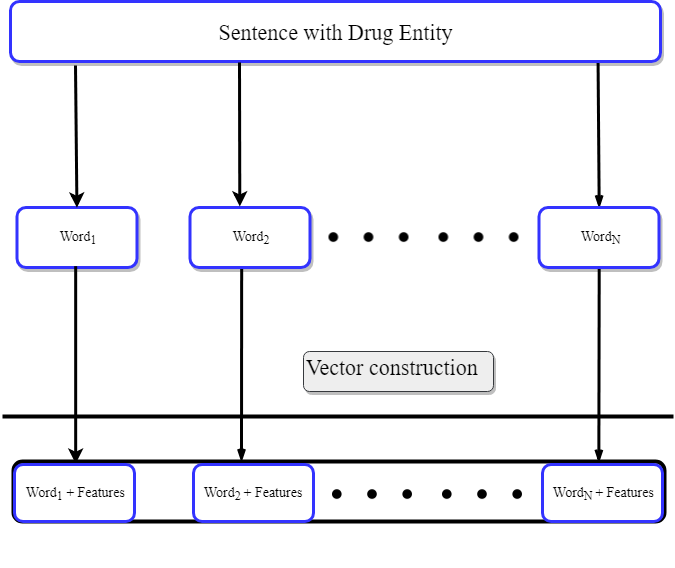
\includegraphics[scale=0.3]{CRF.png}
\end{figure}
\end{frame}

% this is the feature structure used in task 9.1 with the Conditional Random Field learning algorithm.
% We need to feed to the algorithm all the features of all the words of each sentence. In that case, the feataure vector for each individual will contain all those features.


\begin{frame}{Features}{Task9.2 DDI - SVM}
\begin{figure}
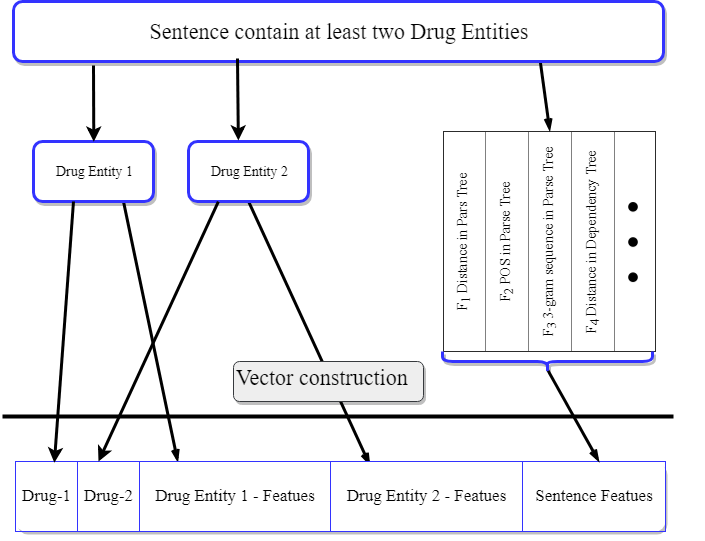
\includegraphics[scale=0.3]{DDI.png}
\end{figure}
\end{frame}


% For the second task to detect drug drug interactions, we have used the single word features for each entity word (in the pair) also with a context window of 3. Then we have added the features derived from the dependency tree (appearances of frequent trigrams, words, lemma, pos. We also added counts of specific POS tags (verbs , determiners, etc).

\section{Experiments}
\begin{frame}{Experiments \& Results}
\begin{center}
\scalebox{0.5}{
\begin{tabular}{ |l|c|c|c|c|c|c|c|c|c|c|c|} 
 \hline
 	Name & Type & Algo. & Features & \# Ftrs & Window & Prec & Rec & F1 & M-Prec & M-Rec & M-F1\\
 \hline
 \rowcolor[HTML]{DAE8FC}
 		\small{ d24tMDmNERaCRFw1m10 } & NER & CRF & pos,ort+pos,ort  &  57 &  -1:+1  &  0.9 & 0.85 & 0.87  &  0.92 & 0.65 & \textbf{0.71} \\
 		\small{ d22btDBmNERaCRFw3m5 } & NER & CRF & pos,ort,lo+pos,ort  &  21 &  -3:+3  &  0.9 & 0.82 & 0.86  &  0.92 & 0.63 & 0.7 \\
 		\small{ d23tDBmNERaLSVMw3m0 } & NER & SVM &
 		
 		\begin{tabular}{c} 
   
 		    lm,pos,lo,chg,ort \\
        
 			+ pos,lo,chg,ort \\ 
 		 \end{tabular}
 			
 			  &  21 &  -2:+2  &  0.83 & 0.79 & 0.81  &  0.64 & 0.54 & 0.58 \\
 		
 		% DrugBank Winner for macro-F1
 		
 		%WBI	3	

 %\hline
 \rowcolor[HTML]{FFCCC9}
 		\small{ SemEval'13	WBI(DrugBank) } & NER &  &   &   &    & 0.921 & 0.914  & 0.917  &  0.653 & 0.659 & \textbf{0.656} \\
\rowcolor[HTML]{FFCCC9}
 		\small{ SemEval'13	UTurku(MedLine) } & NER &  &   &   &    & 0.809 & 	0.521 & 0.634 &  0.649	& 0.528 & \textbf{0.582} \\
 		%remoark our model is overfitted!
 \hline
 
  \rowcolor[HTML]{DAE8FC}
 \small{ ddi006m65(DrugBank) } & DDI & SVM & ort+ort  & 80 &  -3:+3  &  0.6513 & 0.448 & 0.5308  &  0.5778 & 0.3415 & \textbf{0.4293} \\
 		
\small{ ddi006m53(DrugBank) } & DDI & SVM & lm,ort+lm,ort &  96 &  -3:+3  &  0.5748 & 0.4695 & 0.5168  &  0.4292 & 0.3024 & 0.3548 \\

\small{ ddi007m22(MedLine) } & DDI & SVM & 

\begin{tabular}{c} 
   
 		    pos,ort+sent \\
        
 			+ tw,tri,tl,tp \\ 
 		 \end{tabular}
 

                                &  113 &  -3:+3  &  03492 & 02316 & 0.2785  &  05099 & 02531 & 0.3383 \\

 
	
	
 \rowcolor[HTML]{FFCCC9}
\small{ SemEval'13	FBK-irst(DrugBank) } & DDI &  &   &  & &  0.816	& 0.838	& 0.827   &  0.708 &	0.639 &	\textbf{0.672} \\
 \rowcolor[HTML]{FFCCC9}
\small{ SemEval'13	FBK-irst(MedLine) } & DDI &  &   &  & & 0.558 &	0.505 &	0.53  &  0.384 &	0.514 & \textbf{0.44} \\
 		
 		


\hline
 
\end{tabular}
}
\end{center}
\end{frame}

% We present the best three models for each task. with their partial scores (binary entity recognition) and macro scores. We compare those with the highest scored model in the competition for the macro-scores in each task.
% we obtained a good result for the first task. An important remark is that even if we obtain a slightly better result than the competition winner, we haven't done cross-validation so we can consider this to be biased to the test set.
% For the second task, we couldn't really improve from the 35% macro-F1 score except that we tried to reduce the training set and somehow it improved. We can imagine that imbalances of the classes of the reduced dataset have made this reslult improve to 42% but we doubt that this can generalize well. 
%Again, cross-validation will now be required to select the best model within the ones here presented





% \begin{frame}{Experiments \& Results}
% \begin{center}
% \scalebox{0.5}{
% \begin{tabular}{ |l|c|c|c|c|c|c|c|c|c|c|c|} 
%  \hline
%  	Name & Type & Algo. & Features & \# Ftrs & Window & Prec & Rec & F1 & M-Prec & M-Rec & M-F1\\
%  \hline
%  		\small{ m10(MedLine) } & NER & CRF & pos,ort+pos,ort  &  57 &  -1:+1  &  0.9 & 0.85 & 0.87  &  0.92 & 0.65 & 0.71 \\
%  		\small{m5(DrugBank) } & NER & CRF & pos,ort,lo+pos,ort  &  21 &  -3:+3  &  0.9 & 0.82 & 0.86  &  0.92 & 0.63 & 0.7 \\
%  		\small{ m0(DrugBank) } & NER & LSVM & lm,pos,lo,chg,ort+pos,lo,chg,ort  &  21 &  -2:+2  &  0.83 & 0.79 & 0.81  &  0.64 & 0.54 & 0.58 \\
 		
%  		% DrugBank Winner for macro-F1
 		
%  		%WBI	3	

%  \hline			
%  		\small{ SemEval'13	WBI } & NER &  &   &   &    & 0.921 & 0.914  & 0.917  &  0.653 & 0.659 & 0.656 \\
 		
%  		%remoark our model is overfitted!
%  \hline
 
%  \small{ dd65(DrugBank) } & DDI & LSVM & +  &  0 &  :  &  0,6513 & 0,448 & 0.5308  &  0,5778 & 0,3415 & 0.4293 \\
 		
% \small{ dd44(DrugBank) } & DDI & LSVM & +  &  0 &  :  &  0,523 & 0,4762 & 0.4985  &  0,4129 & 0,3122 & 0.3556 \\

% \small{ ddim24(MedLine) } & DDI & LSVM & +  &  0 &  :  &  0,3492 & 0,2316 & 0.2785  &  0,5099 & 0,2531 & 0.3383 \\

% \hline 
	
	

% \small{ SemEval'13	FBK-irst } & DDI &  &   &  & &  0.816	& 0.838	& 0.827   &  0.708 &	0.639 &	0.672 \\
 		

% \hline
 
% \end{tabular}
% }
% \end{center}
% \end{frame}



% \begin{frame}{Experiments \& Results}
% \begin{center}
% \scalebox{0.5}{
% \begin{tabular}{ |l|c|c|c|c|c|c|} 
%  \hline
%  	Name & Type & Algo. & Features & \# Ftrs & Window & Scores \\
%  \hline

%  			\small{ d24tMDmNERaCRFw1m10 } & NER & CRF & pos,ort+pos,ort  &  57 &  -1:+1  &  
 		
%  		\begin{tabular}{|c|c|c|} 
%  			\hline   
%  			P & R & F1  \\
%  			\hline 
%  			0.9 & 0.85 & 0.87 \\ 
%  			\hline  
%  			macro-P & macro-R & \textbf{macro-F1} \\ 
%  			\hline 
%  			0.92 & 0.65 & \textbf{ 0.71 } \end{tabular} \\
%  			\hline 
 		

%  		\small{ d22tDBmNERaCRFw5m5 } & NER & CRF & pos,lo,chg,ort+pos,lo,chg,ort  &  231 &  -5:+5  &  
 		
%  		\begin{tabular}{|c|c|c|} 
%  			\hline   
%  			P & R & F1  \\
%  			\hline 
%  			0.9 & 0.86 & 0.88 \\ 
%  			\hline  
%  			macro-P & macro-R & \textbf{macro-F1} \\ 
%  			\hline 
%  			0.67 & 0.62 & \textbf{ 0.64 } \end{tabular} \\
%  			\hline 
 		
 	
 		
% 		\small{ d23tDBmNERaLSVMw3m0 } & NER & LSVM & lm,pos,lo,chg,ort+pos,lo,chg,ort  &  21 &  -2:+2  &  
		
% 		\begin{tabular}{|c|c|c|} 
% 			\hline   
% 			P & R & F1  \\
% 			\hline 
% 			0.83 & 0.79 & 0.81 \\ 
% 			\hline  
% 			macro-P & macro-R & \textbf{macro-F1} \\ 
% 			\hline 
% 			0.64 & 0.54 & \textbf{ 0.58 } \end{tabular} \\
% 			\hline 
		
%  \hline	
 
  		
% 		\small{ SemEval'13	WBI} & NER &  &   &   &    &  
		
% 		\begin{tabular}{|c|c|c|} 
% 			\hline   
% 			P & R & F1  \\
% 			\hline 
% 		    0.921 & 0.914  & 0.917 \\ 
% 			\hline  
% 			macro-P & macro-R & \textbf{macro-F1} \\ 
% 			\hline 
% 			 0.653 & 0.659 &  \textbf{ 0.656 } \end{tabular} \\
% 			\hline 
		

%  \hline
 
% %  		\small{ SemEval'13	WBI } & NER &  &   &   &    & 0.921 & 0.914  & 0.917  &  0.653 & 0.659 & 0.656 \\
 		
% %  		%remoark our model is overfitted!
% %  \hline
 
% %  \small{ ddi006m65(DrugBank) } & DDI & LSVM & +  &  0 &  :  &  0,6513 & 0,448 & 0.5308  &  0,5778 & 0,3415 & 0.4293 \\
 		
% % \small{ ddi006m44D(DrugBank) } & DDI & LSVM & +  &  0 &  :  &  0,523 & 0,4762 & 0.4985  &  0,4129 & 0,3122 & 0.3556 \\

% % \small{ ddi007m24notop(MedLine) } & DDI & LSVM & +  &  0 &  :  &  0,3492 & 0,2316 & 0.2785  &  0,5099 & 0,2531 & 0.3383 \\

% % \hline 
	
	

% % \small{ SemEval'13	FBK-irst } & DDI &  &   &  & &  0.816	& 0.838	& 0.827   &  0.708 &	0.639 &	0.672 \\
 		

% \hline
% \end{tabular}
% }
% \end{center}
% \end{frame}





\section{Conclusion}
\begin{frame}{Conclusion}{Future work}
Proposed improvements:
\begin{itemize}
    \item Word embedding - use a more suitable ready-made word2vec db or finish clustering.
    \item feature selection by frequency of appearance in the dataset, or entropy computation
    \item model selection by cross-validation
    %\item Train and examine models based on sequential forward selection of features.
    \item use neural network as a learner
\end{itemize}


\end{frame}


\begin{frame}[allowframebreaks]
        \frametitle{References}
        \nocite{*}
        \bibliographystyle{unsrt}
        \bibliography{references}
\end{frame}

\end{document}


